\chapter{入门}

\section{Hello, World!}
\begin{example}[h]
\LoadCode[numbers=left]{texlet/hello-world}
\caption{Hello, World!}
\label{exa:helloworld}
\end{example}

在编辑器中将 \autoref{exa:helloworld} 中的代码保存为 \verb|hello-world.tex|,这就是一份最简单的 \LaTeX 源文件。然后我们可以用 \texttt{xelatex} 程序编译源文件生成 PDF,它知道输入的是 \LaTeX 源文件,所以这里的 \texttt{.tex} 后缀可以省略。以后类似情况都用括号标出,不再特意声明。

\begin{Code}[]
xelatex hello_world(.tex)
\end{Code}

如果系统显示类似下面的错误信息,请检查源文件中是否有拼写错误。\texttt{.log} 文件里有更详细的编译信息。

\begin{Code}[numbers=left]
! LaTeX Error:
...
! Emergency stop.
...
No pages of output.
Transcript written on hello_world.log.
\end{Code}

如果编译成功,系统会报出类似下面的信息:

\begin{Code}[]
Output written on hello_world.pdf (1 page).
Transcript written on hello_world.log.
\end{Code}

\TeX 系统针对不同格式和引擎的组合,提供了一系列的命令行程序,完成不同的编译和转换功能。比如源文件是 plain \TeX 格式时,可以分别用 \texttt{tex, pdftex, xetex} 程序调用 \TeX, pdfTeX, \XeTeX 引擎;源文件是 \LaTeX 格式时,相应的程序则是 \texttt{latex, pdflatex, xelatex} \footnote{现在的发行包大多以pdfTeX为缺省引擎,所以 \texttt{latex} 命令缺省调用的其实是 pdfTeX,而不是 \TeX 。}。选择编译和转换程序时可以参考 \autoref{fig:compile},一般有直接方法可用时,不必非要排个转折亲使用间接方法。

\begin{figure}[htbp]
\centering
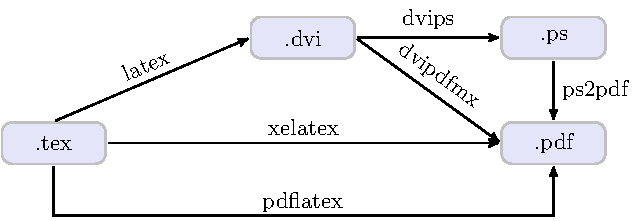
\includegraphics{pgf.pdf}
\caption{编译和格式转换}
\label{fig:compile}
\end{figure}

\section{语法和结构}\label{sec:structure}

\subsection{语法}

\LaTeX 源文件的语句可以分为三种:命令 (command) 、数据和注释 (comment) 。
命令又分为普通命令和环境 (environment) 。普通命令以 \verb|\| 起始,大多只有一行;而环境包含一对起始声明和结尾声明,一般用于多行内容的场合。命令和环境可以互相嵌套。数据就是普通内容。注释语句以 \verb|%| 起始,它在编译过程中被忽略。

比如在 \autoref{exa:helloworld} 中,第1行是注释,第2行是普通命令;第
3, 5行是环境的起始和结尾声明;第4行是数据。

\subsection{物理结构}

\LaTeX 文档的结构可以分为物理结构和逻辑结构。前者指的是源文件的组织形式,包括序言 (preamble) 和正文两部分;后者则是最终输出文档的结构,包括标题、目录、章节等。这里只简要介绍一些基本概念,在第十章还会展开详谈。

序言用来完成一些设置,比如指定文档类型,引入宏包,定义命令、环境等;文档的实际内容则放在正文部分。它们的基本用法如下:

\begin{Code}[]
\documentclass[options]{class}  %文档类声明
\usepackage[options]{package}   %引入宏包
...
\begin{document}                %正文
...
\end{document}
\end{Code}

常用的文档类 (documentclass) 有三种:\texttt{article, report, book},它们的基本选项见 \autoref{tab:class_options}。

\begin{table}[htbp]
\centering
\caption{文档类常用选项}
\label{tab:class_options}
\begin{tabularx}{350pt}{lX}
  \toprule
  10pt, 11pt, 12pt & 正文字号,缺省10pt。\LaTeX 会根据正文字号选择标题、上下标等的字号。\\
  letterpaper, a4paper & 纸张尺寸,缺省是 letterpaper。\\
  notitlepage, titlepage & 标题后是否另起新页。article 缺省 notitlepage,report 和 book 缺省有 titlepage。\\
  onecolumn, twocolumn & 栏数,缺省单栏。\\
  oneside, twoside & 单面双面。article 和 report 缺省用单面,book 缺省用双面。\\
  landscape & 横向打印,缺省是纵向。\\
  openany, openright & 此选项只用于 report 和 book。report 缺省 openany,book 缺省 openright。\\
  draft & 草稿模式。有时某些行排得过满,draft 模式可以在它们右边标上粗黑线提醒用户。\\
  \bottomrule
\end{tabularx}
\end{table}

\LaTeX 核心只提供基本功能,很多功能要通过宏包来实现。其他一些编程语言也有类似的模块化机制,比如 C/C++的 \texttt{include},Java 的 \texttt{import}。

\subsection{逻辑结构}

一份文档的开头通常有标题、作者、摘要等信息,之后是章节等层次结构,内容则散布于层次结构之间。文档比较长时我们还可以使用目录。

标题、作者、日期等命令用法如下,注意 \verb|\maketitle| 命令要放在最后。

\begin{Code}[]
\title{LaTeX Notes}
\author{Alpha Huang}
\date{\today}
\maketitle
\end{Code}

article和report可以有摘要,book里没有。摘要环境用法如下:

\begin{Code}[]
\begin{abstract}
...
\end{abstract}
\end{Code}

\LaTeX 提供了七种层次结构命令,每个高级层次可以包含若干低级层次。article 中没有 chapter,而 report 和 book 则支持所有层次。

\begin{example}[h]
\begin{Code}[numbers=left]
\part{...}          %Level -1
\chapter{...}       %Level 0
\section{...}       %Level 1
\subsection{...}    %Level 2
\subsubsection{...} %Level 3
\paragraph{...}     %Level 4
\subparagraph{...}  %Level 5
\end{Code}
\caption{层次结构}
\label{tab:structure}
\end{example}

我们可以用 \verb|\tableofcontents| 命令来生成目录。系统会自动设定目录包含的章节层次,用户也可以显式指定目录层次深度。比如下面的命令指定目录深度为2,也就是只显示 subsection 及以上层次的目录。注意设定目录深度命令要放在列目录命令的前面。

\begin{Code}[]
\setcounter{tocdepth}{2} %设定目录深度
\tableofcontents         %列出目录
\end{Code}

初次使用目录,或章节图表等层次结构发生变化时,都需要执行两遍编译命令才能获得正确结果。\LaTeX 之所以设计成这样是因为当时的电脑内存容量有限。

如果我们不想让某些层次的标题出现在目录里,则可以给 \autoref{tab:structure} 中的命令加上星号。

\begin{Code}[]
\chapter*{...}
\section*{...}
\subsection*{...}
\subsubsection*{...}
\end{Code}

类似地,我们也可以用下面的命令生成插图和表格目录,插图和表格功能将在后面相关章节中介绍。这两种目录也都需要编译两遍才能获得正确结果。

\begin{Code}[]
\listoffigures
\listoftables
\end{Code}

\section{文字}

文档的内容可以分为文本模式和数学模式。前者是缺省工作方式;要输入数学内容则需要特殊命令或环境。本章只涉及文本模式,第四章会介绍数学模式。

\subsection{字符输入}
\label{sec:char_input}

文档中可以输入的文字符号大致可以分为:普通字符、控制符、特殊符号、预定义字符串、注音符号等。

普通字符可以直接输入,而有些字符 (例如\# \$ \% \^{} \& \_ \{ \} \~{} 等) 被用作特殊的控制符,输入时多数需要在前面加个反斜杠 \verb|\| 来转义。而 \verb|\|本身则要用 \verb|\textbackslash| 命令来输入,因为 \verb|\\| 被用作换行指令\footnote{为什么不用 C 语言的 \verb|\n| 呢,也许因为 \TeX 的编程语言是 Pascal。}。

\begin{Code}[]
\# \$ \^ \& \_ \{ \} \~ \textbackslash \%
\end{Code}

\autoref{tab:symbols} 给出一些特殊符号和预定义字符串的输入方法;其中 \verb|\XeTeX|, \verb|\XeLaTeX| 命令需要 \texttt{metalogo} 宏包,\verb|\MF|, \verb|\MP| 命令需要 \texttt{mflogo} 宏包,\verb|\AmS| 命令需要 \texttt{texnames} 宏包。\autoref{tab:accent} 列出一些注音符号。更多的符号见 Scott Pakin\indexPakin{} \footnote{UIUC 计算机系 1995年硕士,2001年博士。现供职于洛斯阿莫斯国家实验室 (Los Alamos National Laboratory) 。} 的符号列表\citep{Pakin_comprehensive}。

\begin{table}[htbp]
\centering
\caption{特殊符号和预定义字符串}
\label{tab:symbols}
\begin{tabular}{llll}
  \toprule
  \multicolumn{2}{c}{特殊符号} & \multicolumn{2}{c}{预定义字符串} \\
  \cmidrule(lr){1-2} \cmidrule(lr){3-4}
  \textcopyright  & \verb|\textcopyright| & \today & \verb|\today| \\
  {\lmr\textregistered} & \verb|\textregistered|& \TeX  & \verb|\TeX| \\
  {\lmr\texttrademark} & \verb|\texttrademark| & \LaTeX  & \verb|\LaTeX| \\
  \textyen        & \verb|\textyen|       & \LaTeXe  & \verb|\LaTeXe| \\
  \texteuro       & \verb|\texteuro|      & \XeTeX  & \verb|\XeTeX| \\
  \pounds         & \verb|\pounds|        & \XeLaTeX  & \verb|\XeLaTeX| \\
  \dots           & \verb|\dots|          & \MF & \verb|\MF| \\
  \P              & \verb|\P|             & \MP & \verb|\MP| \\
  \S              & \verb|\S|             & \AmS & \verb|\AmS| \\
  \bottomrule
\end{tabular}
\end{table}

\begin{table}[htbp]
\centering
\caption{注音符号}
\label{tab:accent}
\lmr
\begin{tabular}{lp{40pt}lp{40pt}lp{40pt}lp{85pt}}
  \toprule
  \.{A} & \verb|\.{A}| & \"{A} & \verb|\"{A}| & 
    \={A} & \verb|\={A}| & \`{A} & \verb|\`{A}| \\
  \'{A} & \verb|\'{A}| & \^{A} & \verb|\^{A}| & 
    \v{A} & \verb|\v{A}| & \~{A} & \verb|\~{A}| \\
  \d{A} & \verb|\d{A}| & \b{A} & \verb|\b{A}| & 
    \r{A} & \verb|\r{A}| & \textcircled{A} & \verb|\textcircled{A}| \\
  \bottomrule
\end{tabular}
\rmfamily
\end{table}

\LaTeX 中有短划线 (hyphen) 、中划线 (en-dash) 和长划线 (em-dash) 。短划线又称连字符,用来连接单词;中划线用来连接数字,可以通过重复两次短划线得到;长划线类似于中文的破折号,重复三次短划线。为了便于比较,这里也给出数学模式的减号。

\begin{example}[!h]
\begin{RLDemo}[]
computer-aided\\
1840--2010\\
to be---or not to be\\
$1-1=0$
\end{RLDemo}
\caption{划线和减号}
\label{exa:dash}
\end{example}

\subsection{字体样式和大小}
\label{sec:font_style}

拉丁文字体主要有三大类:衬线字体 (roman, serif) 、无衬线字体 (sans serif) \footnote{Sans 这个词来源于法语,就是“没有”的意思。}和等宽字体 (monospace, typewriter) 。衬线字体笔画的边缘部分有些修饰,类似于中文的宋体、仿宋、楷体、魏体等。无衬线字体的笔画则是平滑的,类似于中文的黑体。

字体还可以有粗体 (bold) 、斜体 (italic) 、伪斜体 (oblique, slanted) 、小型大写字母 (small caps) 等修饰效果。\TeX 提供了介于正常字体和粗体之间的半粗体 (medium weight) 。斜体通常对原字体进行了重新设计,它修饰精细,多用于衬线字体;伪斜体基本上是把原字体倾斜,多用于无衬线字体,一般伪斜体看起来比斜体要宽一些。小型大写字母的形状和大写字母相同但尺寸较小,一般高度和小写字母相似。

每种字体样式包含很多种具体的字体,第三章会有关于字体更详细的介绍,包括中文字体的设置。字体常用样式命令见 \autoref{tab:font_style}。

\begin{table}[htbp]
\centering
\caption{字体样式}
\label{tab:font_style}
\begin{tabular}{llll}
  \toprule
  \textrm{roman} & \verb|\textrm{...}| & 
    \textbf{bold face} & \verb|\textbf{...}| \\
  \textsf{sans serif} & \verb|\textsf{...}| & 
    \textmd{medium weight} & \verb|\textmd{...}| \\
  \texttt{typewriter} & \verb|\texttt{...}| & 
    \textit{italic} & \verb|\textit{...}| \\
  \textsc{Small Caps} & \verb|\textsc{...}| & 
    \textsl{slanted} & \verb|\textsl{...}| \\
  \bottomrule
\end{tabular}
\end{table}

\LaTeX 的字体强调命令 \verb|\emph| 在不同字体环境中有不同的效果。如果周围文字是正体,它就是斜体;反之它就是正体。\verb|\underline| 命令可以给字体加下划线,但是它不能正确断字。 \texttt{ulem} 宏包改进了断字,还增加了波浪线和删除线等命令。只是 \texttt{ulem} 把 \verb|\emph| 重定义成了下划线,我们可以在引用宏包时加个选项改回去:\verb|\usepackage[normalem]{ulem}|。

\begin{example}[htbp]
\begin{RLDemo}[]
\emph{emphasis}\\
\uline{underline}\\
\uwave{waveline}\\
\sout{strike-out}
\end{RLDemo}
\caption{字体强调和下划线}
\end{example}

\LaTeX 会根据正文的字体大小来调整标题、章节、上下标、脚注等的字号。我们也可以用 \autoref{tab:fontsize} 中的命令来设置字体相对尺寸,比如正文的字号是10pt, 11pt, 12pt 时,tiny的字号就分别是5pt, 6pt, 6pt。

\begin{table}[htbp]
\centering
\caption{字体相对尺寸}
\label{tab:fontsize}
\begin{tabular}{llrrr}
  \toprule
  & & \multicolumn{3}{c}{正文字号} \\
  \cmidrule(lr){3-5}
  样本 & 命令 & 10pt & 11pt & 12pt \\
  \midrule
  \tiny{sample} & \verb|\tiny|         & 5pt  & 6pt  & 6pt \\
  \scriptsize{sample} & \verb|\scriptsize|   & 7pt  & 8pt  & 8pt \\
  \footnotesize{sample} & \verb|\footnotesize| & 8pt  & 9pt  & 10pt \\
  \small{sample} & \verb|\small|        & 9pt  & 10pt & 11pt \\
  \normalsize{sample} & \verb|\normalsize|   & 10pt & 11pt & 12pt \\
  \large{sample} & \verb|\large|        & 12pt & 12pt & 14pt \\
  \Large{sample} & \verb|\Large|        & 14pt & 14pt & 17pt \\
  \LARGE{sample} & \verb|\LARGE|        & 17pt & 17pt & 20pt \\
  \huge{sample} & \verb|\huge|         & 20pt & 20pt & 25pt \\
  \Huge{sample} & \verb|\Huge|         & 25pt & 25pt & 25pt \\
  \bottomrule
\end{tabular}
\end{table}

\subsection{换行、换页和断字}

通常 \LaTeX 会自动换行,我们也可以用 \verb|\\| 或 \verb|\newline| 命令来强制换行;用 \verb|\newpage| 命令来强制换页。

\LaTeX 也会自动断字 (hyphenate) ,使得每一行的字间距分布均匀。有时我们也需要显式指明断字位置,比如下例就指明 BASIC 这个词不能断开,而 blar-blar-blar 可以在-处断开。

\begin{Code}[]
\hyphenation{BASIC blar-blar-blar}
\end{Code}

\section{长度}
\label{sec:length}

为了精确排版,人们需要控制排版对象的尺寸和位置。\LaTeX 中常用长度单位见 \autoref{tab:unit},其中 point 是个传统印刷业采用的单位,而 big point 是 Adobe 推出 PostScript 时定义的新单位。em 是个相对单位,比如当前字体是 11pt 时,1em 就是 11pt;ex 和 mu 也是相对单位。

\begin{table}[htbp]
\caption{常用长度单位}
\label{tab:unit}
\centering
\begin{tabular}{llllll}
  \toprule
  in & 英寸 & pt & point, 1/72.27 in  & em & 当前字体中字母M的宽度 \\
  cm & 厘米 & bp & big point, 1/72 in & ex & 当前字体中字母x的高度 \\
  mm & 毫米 & pc & pica, 12 pt        & mu & math unit,1/18 em \\
  \bottomrule
\end{tabular}
\end{table}

\LaTeX 为排版对象的尺寸和位置定义了一系列宏变量,以便在排版时重用。我们可以用下面的方法来改变宏变量的值或定义新的宏变量,

\begin{Code}[]
\setlength{`变量名`}   %设置变量的值
\addtolength{`变量名`} %增加变量的值
\newlength{`变量名`}   %定义新变量
\end{Code}

\section{对齐和间距}

\subsection{段落对齐}

\LaTeX 中的段落缺省两端对齐 (fully justified) ,下面的三个环境可以让段落分别居左、居右或居中对齐。

另有三个命令 \verb|\raggedright|、\verb|\centering|、\verb|\raggedleft| 也可以完成同样功能。

\begin{example}[h]
\LoadFRLDemo[]{texlet/par-left}
\LoadFRLDemo[]{texlet/par-right}
\LoadFRLDemo[]{texlet/par-center}
\caption{段落对齐方式}
\end{example}

\subsection{缩进和段间距}
\label{sec:parskip}

\LaTeX 正文中第一个段落缺省不缩进首行,我们可以用 \texttt{indentfirst} 宏包使得第一段也缩进首行。段落首行缩进的距离可以用 \verb|\parindent| 变量来控制,段落之间的距离可以用 \verb|\parskip| 变量来控制。

\begin{Code}[]
\usepackage{indentfirst}
...
\setlength{\parindent}{2em}
\addtolength{\parskip}{3pt}
\end{Code}

\subsection{行间距}
行间距是段落中相邻两行基线之间的距离,\LaTeX 缺省使用单倍行距。我们可以用 \verb|\linespread| 命令来控制行距。

\begin{Code}[]
\linespread{1.3} %一倍半行距
\linespread{1.6} %双倍行距
\end{Code}

\verb|\linespread| 命令不仅会改变正文行距,同时也把目录、脚注、图表标题等的行距给改了。如果只想改正文行距,可以使用 \texttt{setspace} 宏包的行距命令 (见 \autoref{exa:setspace_cmd})。

\begin{example}[h]
\begin{Code}[]
\usepackage{setspace}
...
\singlespacing    %单倍行距
\onehalfspacing   %一倍半行距
\doublespacing    %双倍行距
\setstretch{1.25} %任意行距
\end{Code}
\caption{行距命令}
\label{exa:setspace_cmd}
\end{example}

上述行距命令对全文的行距都会产生影响,\texttt{setspace} 宏包还提供了 \texttt{singlespacing}, \texttt{onehalfspacing}, \texttt{doublespacing} 等环境,可以用来设置局部文字的行距(见 \autoref{exa:setspace_env})。

\begin{example}[h]
\begin{RLDemo}[]
\begin{doublespacing}
double\\spacing
\end{doublespacing}
\end{RLDemo}
\begin{RLDemo}[]
\begin{spacing}{1.25}
any\\spacing
\end{spacing}
\end{RLDemo}
\caption{行距环境}
\label{exa:setspace_env}
\end{example}

\section{特殊段落}
\subsection{摘录}

\LaTeX 中有三种摘录环境:\texttt{quote}, \texttt{quotation}, \texttt{verse}。 \texttt{quote} 两端都缩进, \texttt{quotation} 在 \texttt{quote} 的基础上增加了首行缩进,\texttt{verse} 比 \texttt{quote} 多了第二行起的缩进。

\begin{example}[h]
\LoadFRLDemo[]{texlet/quote-quote}
\LoadFRLDemo[]{texlet/quote-quotation}
\LoadFRLDemo[]{texlet/quote-verse}
\caption{摘录环境}
\end{example}

\subsection{原文打印}
文档中的命令和源代码通常使用等宽字体,也就是原文打印。正文间插入少量等宽文字可以使用 \verb|\verb| 命令;大段原文打印用 \texttt{verbatim} 环境比较方便,它的带星号版本可以标出空格。

\begin{example}[h]
\begin{RLDemo}[numbers=left]
\verb|command| 行间命令
\begin{verbatim}
printf("Hello, world!");
\end{verbatim}
\begin{verbatim*}
printf("Hello, world!");
\end{verbatim*}
\end{RLDemo}
\caption{原文打印}
\end{example}

Timothy van Zandt\indexVanZandt{} \footnote{宾州大学经济系1985年学士,1989年博士。1990年加入普林斯顿,1998年跳到欧洲工商管理学院。} 等人的 \texttt{fancyvrb} 宏包\citep{Zandt_fancyvrb}和 Brooks Moses\indexMoses{} \footnote{1997年弗吉尼亚理工学院机械学士,2007年斯坦福机械博士,毕业后加入一家软件公司源码巫师 (CodeSourcery) 。} 等人的 \texttt{listings} 宏包\citep{Moses_listings}提供了更多的原文打印功能,比如行号、边框、背景、语法着色等。

\subsection{脚注}

脚注可以使用 \verb|\footnote| 命令;如要改变脚注编号形式,可以使用以下命令。
在 \autoref{exa:footnote} 中,\verb|footnote| 是一个计数器 (counter) ;计数器有五种显示格式 (见 \autoref{tab:counter_format}) ,重定义 \verb|\thefootnote| 宏时可任选。

\begin{example}[h]
\LoadFRLDemo[]{texlet/note-footnote}
\begin{Code}[numbers=left]
\renewcommand{\thefootnote}{\roman{footnote}} %i, ii, iii
\end{Code}
\caption{脚注}
\label{exa:footnote}
\end{example}

以后我们还会遇到其他一些计数器,都可以用重定义 \verb|\thecounter| 的方法改变它们的显示格式。

\begin{table}
\centering
\caption{计数器显示格式}
\label{tab:counter_format}
\begin{tabular}{lll}
  \toprule
  阿拉伯数字 & \verb|\arabic{counter}| & 1, 2, 3\dots \\
  小写英文字母 & \verb|\alph{counter}| & a, b, c\dots \\
  大写英文字母 & \verb|\Alph{counter}| & A, B, C\dots \\
  小写罗马数字 & \verb|\roman{counter}| & i, ii, iii\dots \\
  大写罗马数字 & \verb|\Roman{counter}| & I, II, III\dots \\
  \bottomrule
\end{tabular}
\end{table}

原始的脚注命令不能包含原文打印命令或环境,我们可以用 \verb|\texttt| 命令来输入等宽字体,或者用 \texttt{fancyvrb} 宏包的 \verb|\VerbatimFootnotes| 命令重定义 \verb|\footnote| 命令。

\subsection{边注}

边注可以使用 \verb|\marginpar| 命令。单面排版时,边注缺省排在页面右边空白处;双面排版时,边注在外侧,也就是左页的左边或右页的右边;双栏页面的边注排在最近的页边。如要切换边注的方向,可以使用 \verb|\reversemarginpar| 和 \verb|\normalmarginpar| 命令。

\verb|\marginpar| 命令使用浮动体 (float) \footnote{浮动体详见第五章插图和第九章表格。} 来生成边注,所以不能在其他浮动体或脚注内嵌套。 \texttt{marginnote} 宏包的 \verb|\marginnote| 命令不使用浮动体,因而没有这个缺陷。

\begin{example}[h]
\marginnote{正常边注}
\reversemarginpar
\marginnote{反向边注}
\normalmarginpar

\begin{Code}[]
\marginnote{`正常边注`}
\reversemarginpar
\marginnote{`反向边注`}
\normalmarginpar
\end{Code}
\caption{边注}
\end{example}

\subsection{注释}
前面提到可以用百分号来标明注释,但是对于大段文字的注释,百分号就显得比较繁琐 \footnote{有的编辑器提供切换多行百分号的功能,比如TeXNicCenter。}。这时我们可以使用 \texttt{verbatim} 宏包的 \texttt{comment} 环境。

\begin{Code}[]
\begin{comment}
...
\end{comment}
\end{Code}

\section{列表}\label{sec:list}

\subsection{基本列表}

\LaTeX 有三种基本列表环境:无序列表、有序列表、描述列表。这些列表可以单独使用,也可以互相嵌套。

\begin{example}[h]
\subfloat[无序列表]{%
\makebox[\textwidth][l]{%
\LoadRLDemo[numbers=left]{texlet/list-itemize}%
}}\\
\subfloat[有序列表]{%
\makebox[\textwidth][l]{%
\LoadRLDemo[numbers=left]{texlet/list-enumerate}%
}}\\
\subfloat[描述列表]{%
\makebox[\textwidth][l]{%
\LoadRLDemo[numbers=left]{texlet/list-description}%
}}
\caption{基本列表}
\end{example}

\subsection{其他列表}

上述列表的缺省行间距较大,如要节省空间,可以考虑 Bernd Schandl\indexSchandl{}\footnote{1997年凯撒斯劳腾工业大学 (Kaiserslautern University of Technology) 数学硕士,1999年克莱姆森大学数学博士。} 的 \texttt{paralist} 宏包,它提供了一系列压缩列表和行间列表环境。

\begin{example}[!h]
\begin{RLDemo}[numbers=left]
\begin{compactitem}
  \item C++
  \item Java 
  \item HTML
\end{compactitem}
\end{RLDemo}
\begin{RLDemo}[numbers=left]
\begin{compactenum}
  \item C++
  \item Java 
  \item HTML
\end{compactenum}
\end{RLDemo}
\begin{RLDemo}[numbers=left]
\begin{compactdesc}
  \item[C++] 编程语言,
  \item[Java] 编程语言,
  \item[HTML] 标记语言。
\end{compactdesc}
\end{RLDemo}
\caption{压缩列表}
\label{exa:compact_list}
\end{example}

\begin{example}[!h]
\begin{RLDemo}[numbers=left]
\begin{inparaitem}
  \item C++
  \item Java 
  \item HTML
\end{inparaitem}
\end{RLDemo}
\begin{RLDemo}[numbers=left]
\begin{inparaenum}
  \item C++
  \item Java 
  \item HTML
\end{inparaenum}
\end{RLDemo}
\begin{RLDemo}[numbers=left]
\begin{inparadesc}
  \item[C++] 编程语言,
  \item[Java] 编程语言,
  \item[HTML] 标记语言。
\end{inparadesc}
\end{RLDemo}
\caption{行间列表}
\label{exa:inline_list}
\end{example}

%\clearpage
\subsection{定制列表}

如要改变无序列表的列表符号和有序列表的编号形式,可以使用以下代码,其效果见 \autoref{exa:customized_list}。

\begin{Code}[]
\renewcommand{\labelitemi}{-}
\renewcommand{\theenumi}{\alph{enumi}}
\end{Code}

\renewcommand{\labelitemi}{-}
\renewcommand{\theenumi}{\alph{enumi}}

\begin{example}[htbp]
\LoadRLDemo[numbers=left]{texlet/list-itemize}\\
\LoadRLDemo[numbers=left]{texlet/list-enumerate}
\caption{定制列表}
\label{exa:customized_list}
\end{example}

\renewcommand{\labelitemi}{\ensuremath{\bullet}}
\renewcommand{\theenumi}{\arabic{enumi}}

\section{盒子}
\label{sec:box}

\LaTeX 在排版时把每个对象 (小到一个字母,大到一个段落) 都视为一个矩形盒子 (box) ,我们在HTML和CSS中也可以见到类似的模型。

\subsection{初级盒子}

最简单的盒子命令是 \verb|\mbox|和 \verb|\fbox|。前者把一组对象组合起来,后者在此基础上加了个边框。

\begin{example}[htbp]
\begin{RLDemo}[]
\mbox{010 6278 5001}
\fbox{010 6278 5001}
\end{RLDemo}
\caption{ \texttt{mbox}和 \texttt{fbox}}
\label{exa:mbox}
\end{example}

\subsection{中级盒子}

稍复杂的 \verb|\makebox| 和 \verb|\framebox| 命令提供了宽度和对齐方式控制的选项。其对齐方式有居中 (缺省) 、居左、居右和分散对齐,分别用 \texttt{c}, \texttt{l}, \texttt{r}, \texttt{s} 来表示。

\begin{example}[htbp]
\LoadFRLDemo[]{texlet/box-make}
\caption{ \texttt{makebox}和 \texttt{framebox}}
\label{exa:makebox}
\end{example}

\subsection{高级盒子}

大一些的对象比如整个段落可以用 \verb|\parbox| 命令或 \texttt{minipage} 环境,两者语法类似,有宽度、高度、外部对齐、内部对齐等选项。这里的外部对齐是指该盒子与周围对象的纵向关系,有三种方式:居顶、居中和居底对齐,分别用 \texttt{t}, \texttt{c}, \texttt{b} 来表示。内部对齐是指该盒子内部内容的纵向排列方式,也是同样三种。

\verb|语法:[外部对齐][高度][内部对齐]{宽度}{内容}|

\begin{example}[htbp]
\LoadCode[numbers=left]{texlet/box-par-esc}
\input{texlet/box-par}
\caption{\texttt{parbox} 和 \texttt{minipage}}
\label{exa:parbox}
\end{example}

%\subsection{彩色盒子}
%\subsection{盒子升降}
%\subsection{盒子存取}

\section{交叉引用}
\label{sec:crossref}

在 \LaTeX 中我们可以任意设置标签,然后引用标签前面最近一个对象 (章、节、图、表等) 的编号或者页码,这就是交叉引用 (cross reference) 。\autoref{exa:ref} 中的 \texttt{marker} 是一个标签名,它在全文中须保持唯一。

\begin{example}[h]
\LoadFBTDemo[]{texlet/ref}% label in example environment doesn't work
\caption{交叉引用}
\label{exa:ref}
\end{example}

文档中新增标签后,第一次编译时会得到类似下面的警告信息。因为第一次编译只会扫描出有标签的地方,第二次编译才能得到正确结果。

\begin{Code}[]
LaTeX Warning: There were undefined references.
LaTeX Warning: Label(s) may have changed. Rerun to get cross-references right.
\end{Code}

\bibliographystyle{unsrtnat}
\bibliography{lnotes2}
